\documentclass[conference]{IEEEtran}

% to enable \thanks
\IEEEoverridecommandlockouts

\usepackage{cite}

\begin{document}

\title{Subsetter}

\author{
\IEEEauthorblockN{
    Jeff Daily\IEEEauthorrefmark{1},
    Karen Schuchardt\IEEEauthorrefmark{1} and
    Bruce Palmer\IEEEauthorrefmark{1}
}
\IEEEauthorblockA{
    \IEEEauthorrefmark{1}
    Pacific Northwest National Laboratory\\
    jeff.daily,karen.schuchardt,bruce.palmer@pnl.gov
}
\thanks{Wei-keng Liao}
}

\maketitle

% For peer review papers, you can put extra information on the cover
% page as needed:
% \ifCLASSOPTIONpeerreview
% \begin{center} \bfseries EDICS Category: 3-BBND \end{center}
% \fi
%
% For peerreview papers, this IEEEtran command inserts a page break and
% creates the second title. It will be ignored for other modes.
\IEEEpeerreviewmaketitle

\begin{abstract}
\label{section:abstract}

The size of datasets produced by current climate models is increasing rapidly
to the scale of petabytes.  To handle data at this scale parallel analysis
tools are required, however the majority of climate analysis software remain
at the scale of workstations.  Further, many climate analysis tools adequately
process regularly gridded data but lack sufficient features when handling
unstructured grids.  This paper presents a data-parallel subsetter capable of
correctly handling unstructured grids while scaling to over 2000 cores.  The
approach is based on the partitioned global address space (PGAS) parallel
programming model and one-sided communication.  The paper demonstrates that IO
remains the single greatest bottleneck for this domain of applications and
that parallel analysis of climate data succeeds in practice.

\end{abstract}

\section{Introduction}
\label{section:introduction}

Parallel programming is needed to analyze the size of output data produced by
today's climate models.\cite{MODSIM07:LOT}  A single snapshot of Randall's
Global Cloud Resolving Model will produce terabytes of data\cite{GCRM}; the
analysis of even a modest time series of this data will quickly overwhelm
today's software and traditional climate analysis systems.  For these data
sizes, I/O bandwidth represents the single greatest bottleneck for analysis
tools.  Parallel software leveraging parallel file systems must be used to
process this data, however current climate analysis tools are at most task
parallel and rely on a single data reader.\cite{CDAT}\cite{CDO}\cite{NCO}

Many climate analysis tools robustly handle the manipulation and display of
regularly gridded data.  However, these same applications lack sufficient
features when handling unstructured or irregular grids such as the geodesic or
cubed sphere\cite{CUBE}.  Unstructured grids are gaining popularity, further
widening the gap between current software and these types of models.  For
unstructured grids it is necessary to provide more information about the
topology of the grid and maintain the integrity of this topology information
in the face of data culling.

Regular grids allow for the topology to be implicitly defined by how
the data is stored; coordinate variables are generally monotonic and cell
neighbors are adjacent both logically and in memory. These assumptions allow
for operations over regular grids which are otherwise more difficult to
perform over unstructured grids. In the case of partitioning these grids for
data parallel processing, unstructured grids will often have more of the
logically adjacent cells scattered across memory partitions than in the
regular case.

Subsetting is a fundamental capability for any analysis tool and allows users
to operate over the regions of the data in which they are interested. The
subsetting operation is useful as part of a larger operation over the data,
such as for obtaining regional averages, but is also useful to post-process
data into a new dataset such that the cost of subsetting can be amortized
across future operations over the same region. Further, as the size of
datasets grow subsetting is important to reduce the data to a size that
traditional analysis tools are capable of handling. 

In this paper, we present a parallel tool for subsetting very large geodesic
climate data in parallel while preserving the explicit topology.  The code is
built using the Global Arrays (GA) toolkit which provides an efficient and
portable "shared-memory" programming interface for distributed-memory
computers and features truly one-sided communications.\cite{GA}  GA
traditionally deals with dense arrays, however its sparse data operations as
well as its one-sided operations allow for efficient subsetting over
unstructured grids.

The primary contributions of the paper are:
\begin{itemize}
\item A parallel subsetter of geodesic data based on the partitioned global address space programming model and one-sided communications
\item A novel algorithm for the maintenance of unstructured grid data
\item A novel algorithm for the subset and even distribution of unstructured grid data
\item Evaluation showing IO to be the greatest bottleneck in scaling these types of applications
\end{itemize}

The paper is organized as follows.  Section \ref{section:requirements}
describes the requirements while \ref{section:design} describes the design of
the subsetter, its algorithms, and how GA's unique features were leveraged.
Section \ref{section:implementation} briefly describes how the subsetter was
implemented.  Section \ref{section:evaluation} presents our experimental design
and the performance characteristics of the subsetter on nearly full-scale data
set sizes of model data up to a resolution of 4Km.  We present the
capabilities under development as well as the capabilities we would like to
see in section \ref{section:future}.  Finally, section
\ref{section:conclusion} presents our conclusions.

\section{Design}
\label{section:design}

In this section we describe the design of our classes and algorithms based on
the requirements established in \ref{section:requirements}.

\subsection{How to Run the Subsetter}

The success of the NetCDF Operators and similar tools demonstrate the need for
user-ready applications for the analysis of their data while the success of
tools such as CDAT validate the need for a scriptable interface and customization of
basic and advanced operators.  We plan to provide both the scriptable
interface as well as a set of predefined tools.

The subsetter is the first in a series of planned parallel command-line tools
based on unstructured grids and the PGAS programming model.  It takes
arguments specifying specific variables (-v) or dimension ranges (-d) to
extract, or at a higher level a latitude and longitude bounding box (-b).  In
this way it is most akin to the NetCDF Operators' "kitchen sink" application.
Example usage looks like: \begin{itemize} \item mpiexec -np 128 subsetter -b
20,-20,160,90 -v vorticity january.nc february.nc MJO\_vorticity\_janfeb.nc
\item mpiexec -np 64 subsetter -b 90,0,180,-180 -d levels,1,5 geopotential.nc
\end{itemize}

\subsection{Dataset Abstraction}

The subsetter minimally supports two forms of input file aggregation, either
across a specified dimension e.g. time or by taking the union of all input
files such that duplicate dimensions and variables within later files are
ignored.  These forms of aggregation are modeled after what is available when
using NetCDF Markup Language.\cite{NcML} NcML input is not directly supported
at this time but is planned for a future release. 

\subsection{Parallel IO Abstraction}

IO operations are hidden behind abstract base classes.  Any IO library can be
supported.  This is similar to how the Java NetCDF library works
\cite{JavaNetCDF}.  Further, differing IO strategies using the same IO library
can also be developed behind the same API.  The use of Parallel NetCDF was
selected because of the ubiquity of the NetCDF libraries and data format in
climate applications.

\subsection{The Global Arrays Library}

The partitioned global address space (PGAS) programming model assumes a global
address space which is partitioned such that each process is associated with a
local portion of the space.  One-sided communication allows a process to
access another process's address space without any explicit participation by
the latter process.  Such communication can reduce synchronization, reduce
data movement, and can simplify programming.  The Global Arrays (GA) library
supports both models.

The subsetter was built using the GA library for the wealth of features it
provides which are tailored to our problem domain.  GA provides a distributed
dense multidimensional array programming abstraction and the data we will be
operating over is stored as dense arrays within NetCDF files.  It should be
noted that dense distributed arrays would also work well for regularly gridded
data.  However, due to the use of unstructured grid data, the algorithm for
subsetting the data will look quite different than for the structured case.
Recall that for unstructured grids, logically adjacent cells are not
necessarily adjacent in memory.  In order to evenly distribute a subset, a
single process will need to send a varying amount of data to any number of
other processes.  Certainly a collective operation could be considered, but GA
provides the necessary functionality without needing any explicit cooperation
from any other process.  Any given process will simply put the section of the
subset into the remote process's memory.

There are certain GA one-sided operations which are tailored for use on
one-dimensional arrays which are prevalent within our data.  These operations
include \verb=GA_Patch_enum=, \verb=GA_Scan_add=, \verb=GA_Scan_copy=,
\verb=GA_Pack=, and \verb=GA_Unpack=.  Those operations have been demonstrated
in the computation of sparse matrix multiplication\cite{GA} but are equally
useful in the manipulation of unstructured grids.  The remaining GA operations
are N-dimensional and include \verb=NGA_Scatter=, \verb=NGA_Gather=,
\verb=GA_Put=.  Those operations are useful for redistributing the subset
data.

\subsection{The Algorithms}

The one-sided communications and PGAS model supported by GA allowed us to
develop some novel algorithms for the manipulation of unstructured grids.  In
this section we diagram and describe the algorithms we developed.  The vast
majority of functionality within the subsetter is provided by either PnetCDF
or GA.  GA allocates and evenly distributes the arrays which are then filled
with data by PnetCDF.  GA operations are then used to prepare the data for
packing at which point a custom n-dimensional packing routine is used.  The
packed, evenly-distributed data is then written back to disk using PnetCDF.
Of these algorithms, the novel ones include reindexing the masks, reindexing
the topology variables, and the n-dimensional pack routine.

Each dimension of the data has two arrays associated with it, a bitmask and an
integer array representing the new indices of the dimension in case of a
subset.  For instance, if any of the bits are turned off, the corresponding
indices of the index array will have negative values.  The remaining values of
the index array will increase monotonically, skipping the negative or masked
indices.  The bitmasks are generated based on a rectangular latitude and
longitude region specified on the command-line, or by specifying one or more
indices of a dimension to select.  Although a rectangular region is currently
used for simplicity, once translated the bitmasks allow for arbitrary subsets
to be defined.  These bitmasks are then used to evenly distribute the
resultant subset across all processes.  Note that these bitmask and associated
index arrays are one-dimensional and distributed.

\subsubsection{Partial Sum}

\begin{figure}[!t]
\center
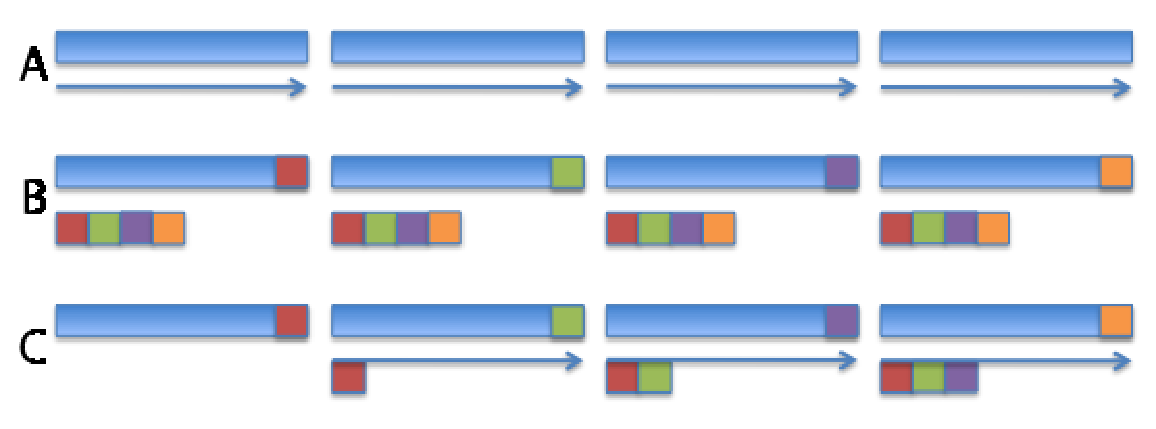
\includegraphics[width=3.5in]{images/partialsum_label}
\caption{Distributed partial sum on a 1-D array}
\label{fig:partialsum}
\end{figure}

A partial sum of the index array associated with each dimension is useful for
later determining where subset data is to be placed.  That feature will be
explained in more detail in \ref{section:alg_pack}.  The partial sum operation
here is semantically similar to the one found in the C++ STL\cite{CXXSTL}.  It
computes a series of sums over an array from the first element through the
\emph{i}th element and stores the result of each such sum in the \emph{i}th
element of a destination array.

The partial sum is computed by first performing partial sums of each local
portion of the source array.  This operation is represented by
\ref{fig:partialsum} A.  The last value of each local sum is then collectively
distributed to each process as seen in \ref{fig:partialsum} B.
\ref{fig:partialsum} C is the last step where each local portion adds the last
values of each process's sum which come before.

\subsubsection{Reindexing of Dimension Index}

\begin{figure}[!t]
\center
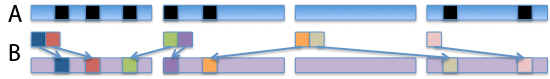
\includegraphics[width=3.5in]{images/unpack_label}
\caption{Reindexing of a Dimension Index}
\label{fig:unpack}
\end{figure}

Creating the index array associated with a mask requires three specific GA
operations, \verb=GA_Fill=, \verb=GA_Patch_enum= and \verb=GA_Unpack=.  The
mask array is represented in \ref{fig:unpack} A.  \verb=GA_Fill= fills the
index array, the bottom array in \ref{fig:unpack} B,  with a value of $-1$.  A
second array is created after each process counts how many masked bits are
present and collectively sums to get the size of the array to create.
\verb=GA_Patch_enum= enumerates the values in the second array starting from
zero with an increment of 1.  The enumerated array is shown in
\ref{fig:unpack} B.  \verb=GA_Unpack= expands the enumerated array values into
the filled array based on the associated mask array, seen as \ref{fig:unpack}
B.

\subsubsection{Reindexing of Topology Variables}

\begin{figure}[!t]
\center
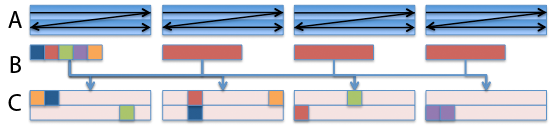
\includegraphics[width=3.5in]{images/reindex_label}
\caption{Reindexing of Topology Variables}
\label{fig:reindex}
\end{figure}

Recall that the topology variables are those which map from one index to
one or more other indices such as from a cell index to each of its corner
indices.  A typical subset operation reduces the number of cells, corners, and
edges within the grid, so it is important to maintain the integrity of these
mapping arrays such that they map to real indices.

The reindexing of the topology variables relies on the recalculated index
array of the associated domain.  For example, when reindexing the mapping from
edges to corners, the recalculated corners index array is required.  The
mapping values represent indices into the recalculated index array.  The
mapping arrays are iterated over to gather the required indices for the
subsequent GA routine \verb=NGA_Gather= to query, represented in
\ref{fig:reindex} A.  The \verb=NGA_Gather= routine gathers array elements
from a global array into a local array.  In this each process gathers the new
values for the mapping from the index array (\ref{fig:reindex} B) and
then appropriately replaces the old mapping values in \ref{fig:reindex} C.

\subsubsection{N-Dimensional Pack}
\label{section:alg_pack}

\begin{figure}[!t]
\center
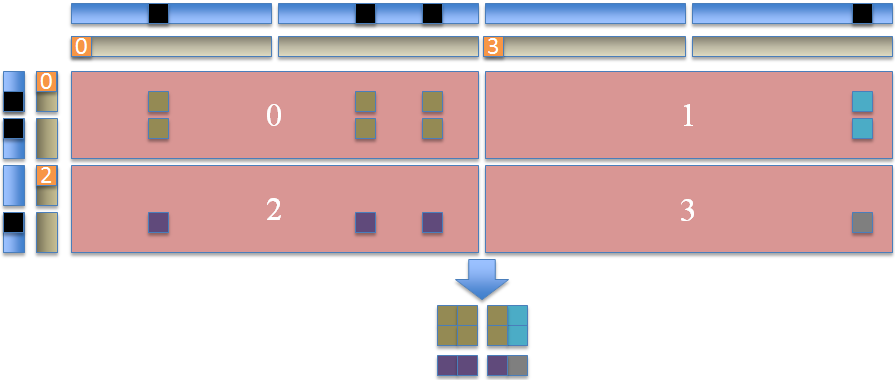
\includegraphics[width=3.5in]{images/pack}
\caption{Pack}
\label{fig:pack}
\end{figure}

The goal of the pack routine is to evenly distribute the subset destination
array from the already evenly distributed source array.  The subset is
specified using mask arrays, one for each dimension of the source array.  The
problem lies with where to put the data once each process computes its portion
of the subset; each process would need to know a priori the size of the
subsets that logically come before their own computed portion and
\verb=NGA_Put()= their data after then.

The partial sum of the mask array is a convenient solution to this problem.
Each process owns a portion of the source array in terms of the global address
space of the array.  For each dimension, the value in the corresponding
partial sum array at the index represented by the lowest index owned by each
local portion describes where to put the subset data.

Figure \ref{fig:pack} should clarify this.  In the figure, the blue arrays
represent both the mask arrays as well as the partial sum arrays.  The masked
bits are indicated in black.  Each of the four processes query the partial sum
arrays using \verb=NGA_Get()= at the corresponding locations indicated in
orange and the small blue arrows.  Now knowing where to put their subset data,
each process can \verb=NGA_Put()= their portions resulting in the subset
array.

\section{Results}
\label{section:results}

TODO

\section{Future Work}
\label{section:future}

The success of the NetCDF Operators\cite{NCO} and similar tools demonstrate
the need for user-ready applications for the analysis of their users' data.
The success of tools such as CDAT\cite{CDAT} validate the need for a
scriptable interface and customization of basic and advanced operators.  We
plan to provide both the scriptable interface as well as a set of predefined
command-line tools.

We are currently developing a general C++ API for climate data analysis in a
data parallel fashion based on the PGAS model and one-sided communications.
The API will be leveraged to produce additional command-line tools, however it
is intended primarily to be used by climate scientists to produce the kinds of
tailored analyses which they require.  Time permitting, the API will be
exposed to the Python language in order to facilitate ease of use in a
scripted environment.  Larson, Ong, and Tokarz also point out certain
capabilities missing from popular climate data analysis packages such as
probability density function (PDF) estimation as well as the sorting and
ordering of data.

The evaluation performed in Section \ref{section:evaluation} revealed that IO
for our application remains the greatest bottleneck.  This fact is exacerbated
when large regions representing the entire grid are subset.  Our current
optimized strategy of reading chunks of variables based on whether a process
participates in the later subset still reads more data than is eventually
redistributed.  If a masked read or a read based on individual array index
tuples similar to \verb+NGA_Gather+ were available within the Parallel-NetCDF
library we might see further performance gains.  The algorithms presented in
this paper which evenly distribute the subset data will hopefully encourage
work in this area.  We are also investigating recent advances in the
Parallel-NetCDF library \cite{PNETCDFOPT} which addresses the limitation in
the current interface of only allowing access to one array variable per
function call.

\section{Conclusion}
\label{section:conclusion}

We developed a novel data parallel subsetter of climate data based on
unstructured grids, the PGAS programming model, and one-sided communication.
The experimental evaluation showed scalability to thousands of processors and
acceptable IO bandwidth.  IO bandwidth is the greatest bottleneck in scaling
these types of applications.

\section*{Acknowledgment}
The authors are indebted to Wei-keng Liao at Northwestern University for
invaluable help in getting the subsetter running and optimized on the Franklin
platform.

This research was funded by the U.S. Department of Energy's (DOE) Office of
Advanced Scientific Computing Research through its Scientific Discovery
through Advanced Computing program and was performed at DOE's National Energy
Research Scientific Computing Center.


% trigger a \newpage just before the given reference
% number - used to balance the columns on the last page
% adjust value as needed - may need to be readjusted if
% the document is modified later
%\IEEEtriggeratref{8}
% The "triggered" command can be changed if desired:
%\IEEEtriggercmd{\enlargethispage{-5in}}

% references section

\bibliographystyle{IEEEtran}
\bibliography{IEEEabrv,paper}

% that's all folks
\end{document}
